\begin{figure*}[t]
\centering
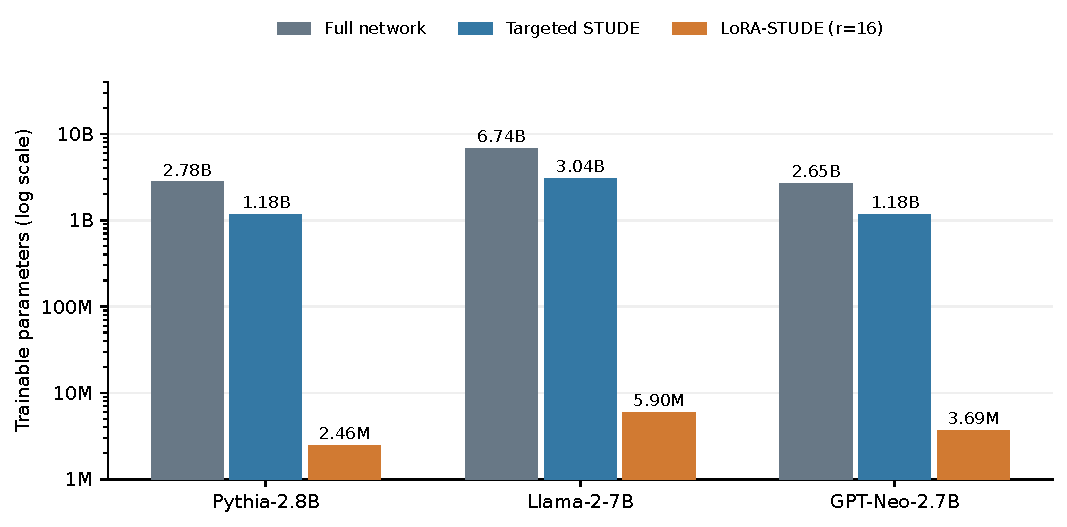
\includegraphics[width=0.9\textwidth]{figures/parameter_budget/parameter_budget.pdf}
\caption{Trainable parameter counts for full-network updates, targeted STUDE (all block parameters in zero-indexed layers 10--24, inclusive), and LoRA-STUDE (rank 16, attention Q/K/V in the same layers; fused QKV for Pythia). Counts come from configuration-only meta-device models and actual PEFT adapter insertion; tied weights are counted once. Frozen base weights remain resident for LoRA. Counts describe gradient-update scope, not total model storage, runtime, optimizer memory, or the number of nonzero weights. The preliminary pruning edit is excluded. Full-network is a reference update scope, not a measured DEL or SPE budget.}
\label{fig:parameter-budget}
\end{figure*}
